\subsection{Schedule}

Scheduling of the project is presented in a Gantt Chart overview on Figure \ref{fig:schedule-gantt-chart}. Exam period constraints have been included in order to evaluate risks in person-day allocations to project implementation. It is expected during exam periods the team work output will be lower than usual but project activities will continue, therefore time has been planned accordingly to accommodate this:

\begin{figure}[H]
    \begin{align*}
        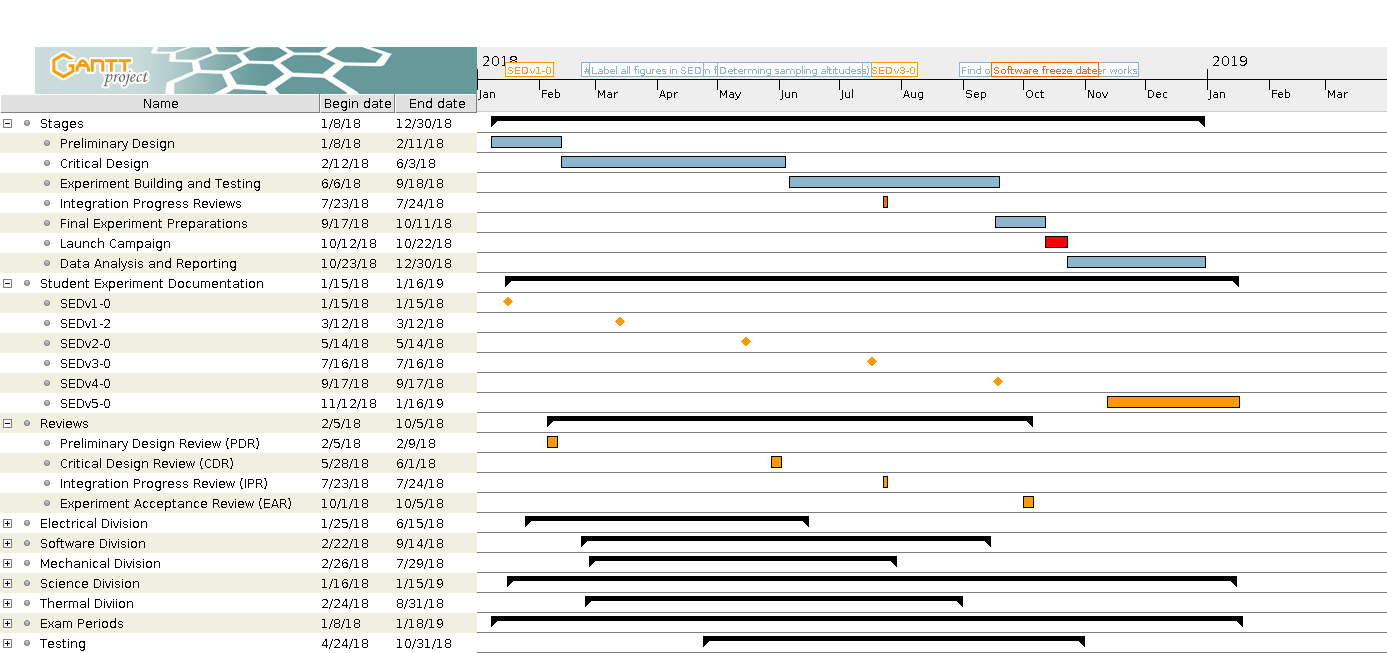
\includegraphics[width=1\linewidth]{3-project-planning/img/BEXUS-SED-GanttChart-Overview.png}
    \end{align*}
    \caption{Project Schedule Gantt Chart.}\label{fig:schedule-gantt-chart}
\end{figure}

Deadlines of the five Student Experiment Documentations (SED) versions have been estimated based on past REXUS/BEXUS Cycles. An expanded version of the Gantt Chart with detailed listing of all sub-tasks not shown in Figure \ref{fig:schedule-gantt-chart} can be found in Appendix \ref{sec:appF}. This expanded Gantt Chart includes all tasks related to the test plan and internal deadlines are set so that a first draft of the documentation is completed one week in advance to allow contents to be checked. Build and test internal deadlines are also placed one week in advance to allow a buffer in case things do not go as expected. The tests are scheduled for as early as possible to allow time for rescheduling if the result is a fail. With some high priority tests, see Section \ref{sec:5.2.1-testpriority}, it is expected these will be very difficult to reschedule therefore extra time is built into the test duration to allow for multiple attempts at the test.

